\documentclass{sintefbeamer}
\usepackage{multicol}
\usepackage{animate}
\usepackage{booktabs}
\usetikzlibrary{arrows.meta, positioning}
\usetikzlibrary{calc}

% --- پشتیبانی فونت فارسی (XePersian + Vazirmatn) ---
\usepackage[extrafootnotefeatures]{xepersian}
\settextfont[Path=./font/, BoldFont=Vazirmatn-Bold.ttf]{Vazirmatn-Regular.ttf}
\setlatintextfont[Path=./font/, BoldFont=Vazirmatn-Bold.ttf]{Vazirmatn-Regular.ttf}
% --- پایان افزوده ---

% شکل‌های ارائه از reports/figures/ مخزن می‌آیند، نه از images/ محلی
\graphicspath{%
  {images/}%
  {../reports/figures/slides/}%
  {../reports/figures/}%
  {../reports/figures/phase8/}%
  {../reports/figures/phase9/}%
  {../reports/figures/phase10/}%
  {../reports/figures/round4/}%
  {../reports/figures/round5/}%
}

% meta-data
\title{بهینه‌سازی پیش‌بینی میزان پخت غذا در سلف‌های دانشگاه تهران}
\subtitle{ارائه به استاد راهنما}
\author{مهدی وجهی}
\institute{دانشکده مهندسی برق و کامپیوتر، دانشگاه تهران \\ استاد راهنما: دکتر بابک نجار اعرابی}
\date{شهریور ۱۴۰۵}
\setbeamertemplate{footline}[frame number]

% document body
\begin{document}

\maketitle


\section{Introduction to NN}


\begin{frame}{Neural Networks}
  
  \begin{figure}
    \centering
    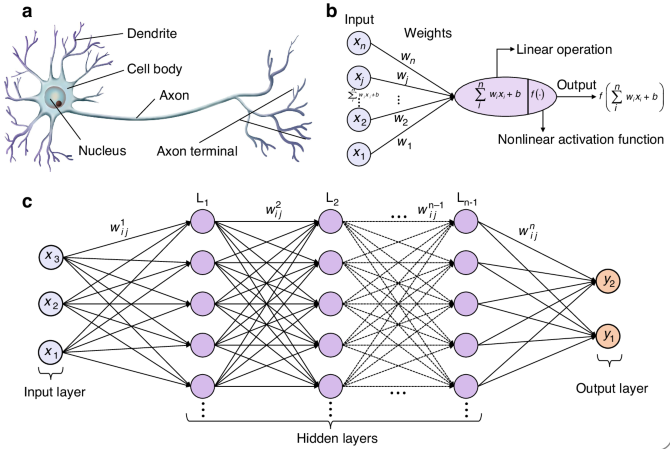
\includegraphics[width=0.85\textwidth]{images/41377_2024_1590_Fig3_HTML.png}
  \end{figure}

\end{frame}

\begin{frame}{Networks for AND logic}
  \begin{multicols}{2}
\begin{center}
  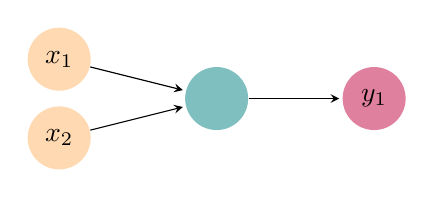
\begin{tikzpicture}[>=stealth]
% \centering
% Parameters
\def\inputnum{2}
\def\hiddennum{1}
\def\outputnum{1}

% Input Layer
\foreach \i in {1,...,\inputnum}
{
	\node[circle, minimum size=8mm, fill=orange!30] 
		(Input-\i) at (2,-\i) {$x_{\i}$};
}

% Hidden Layer
\foreach \i in {1,...,\hiddennum}
{
	\node[circle, minimum size=8mm, fill=teal!50,
		yshift=(\hiddennum-\inputnum)*5 mm]
		(Hidden-\i) at (4,-\i) {};
}

% Output Layer
\foreach \i in {1,...,\outputnum}
{
	\node[circle, minimum size=8mm, fill=purple!50,
		yshift=(\outputnum-\inputnum)*5 mm]
		(Output-\i) at (6,-\i) {$y_{\i}$};
}

% Connect neurons In-Hidden
\foreach \i in {1,...,\inputnum}
{
	\foreach \j in {1,...,\hiddennum}
	{
		\draw[->, shorten >=1pt] (Input-\i) -- (Hidden-\j);	
	}
}

% Connect neurons Hidden-Out
\foreach \i in {1,...,\hiddennum}
{
	\foreach \j in {1,...,\outputnum}
	{
		\draw[->, shorten >=1pt] (Hidden-\i) -- (Output-\j);
	}
}
\end{tikzpicture}
$$ y_1 = f(w_1 x_1 + w_2 x_2 + b)$$


    \begin{table}[h!]
    % \centering
    \begin{tabular}{|c|c|c|}
      \hline
      $x_1$ & $x_2$ & $y_1= x_1\land x_2 $ \\ 
      \hline
      0 & 0 & 0 \\ 
      0 & 1 & 0 \\ 
      1 & 0 & 0 \\ 
      1 & 1 & 1 \\ 
      \hline
    \end{tabular}
   
  \end{table}


  \vspace{0.5cm}
  \pause
  $$f(x) = \frac{1}{1+e^{-x}}$$
  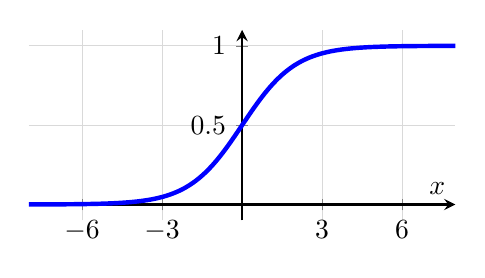
\begin{tikzpicture}
  \begin{axis}[
      axis lines = middle,
      samples = 200,
      domain = -8:8,
      width = 7cm,
      height = 4cm,
      xlabel = {$x$},
      % ylabel = {$f(x)$},
      ymin = -0.1, ymax = 1.1,
      grid = both,
      major grid style={gray!30},
      minor grid style={gray!10},
      thick,
      smooth,
      xtick={-6,-3,0,3,6},
      ytick={0,0.5,1}
    ]
    \addplot[blue, ultra thick, domain=-8:8]
      {1/(1+exp(-x))};
  \end{axis}
\end{tikzpicture}

\end{center}


  \end{multicols}

\end{frame}

\begin{frame}{Networks for AND logic}
\begin{equation*}
   y_1 = f(5.5 x_1 + 5.5 x_2 -8)
\end{equation*}
\begin{table}[h!]
\centering

\centering
\begin{tabular}{|c|c|c|c|c|}
\hline
$x_1$ & $x_2$ & Weighted Sum & $f(\text{sum})$ & Output \\ 
\hline
0 & 0 & -8.0 & 0.0003 & 0 \\ 
0 & 1 & -2.5 & 0.075  & 0 \\ 
1 & 0 & -2.5 & 0.075  & 0 \\ 
1 & 1 & 3.0  & 0.952  & 1 \\ 
\hline
\end{tabular}
\caption{Neural network output for AND operation.}

\hfill

\end{table}

\end{frame}

\begin{frame}{Training a Neural Networks}
\begin{center}
  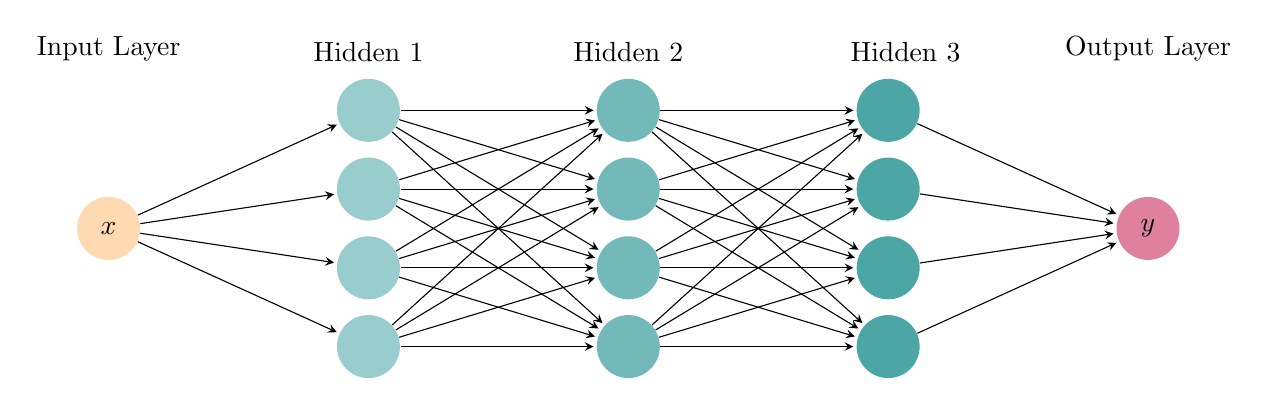
\begin{tikzpicture}[>=stealth, x=2.2cm, y=1cm]
\centering
% Parameters
\def\inputnum{1}
\def\hiddennum{4}
\def\outputnum{1}

% === Input Layer ===
\foreach \i in {1,...,\inputnum}{
  \node[circle, minimum size=8mm, fill=orange!30] 
    (Input-\i) at (0,-\i-1) {$x$};
}

% === Hidden Layer 1 ===
\foreach \i in {1,...,\hiddennum}{
  \node[circle, minimum size=8mm, fill=teal!40] 
    (HiddenA-\i) at (1.5,-\i + 0.5) {};
}

% === Hidden Layer 2 ===
\foreach \i in {1,...,\hiddennum}{
  \node[circle, minimum size=8mm, fill=teal!55] 
    (HiddenB-\i) at (3,-\i + 0.5) {};
}

% === Hidden Layer 3 ===
\foreach \i in {1,...,\hiddennum}{
  \node[circle, minimum size=8mm, fill=teal!70] 
    (HiddenC-\i) at (4.5,-\i + 0.5) {};
}

% === Output Layer ===
\foreach \i in {1,...,\outputnum}{
  \node[circle, minimum size=8mm, fill=purple!50]
    (Output-\i) at (6,-\i-1) {$y$};
}

% === Connections ===
% Input → Hidden 1
\foreach \i in {1,...,\inputnum}{
  \foreach \j in {1,...,\hiddennum}{
    \draw[->, shorten >=1pt] (Input-\i) -- (HiddenA-\j);
  }
}

% Hidden 1 → Hidden 2
\foreach \i in {1,...,\hiddennum}{
  \foreach \j in {1,...,\hiddennum}{
    \draw[->, shorten >=1pt] (HiddenA-\i) -- (HiddenB-\j);
  }
}

% Hidden 2 → Hidden 3
\foreach \i in {1,...,\hiddennum}{
  \foreach \j in {1,...,\hiddennum}{
    \draw[->, shorten >=1pt] (HiddenB-\i) -- (HiddenC-\j);
  }
}

% Hidden 3 → Output
\foreach \i in {1,...,\hiddennum}{
  \foreach \j in {1,...,\outputnum}{
    \draw[->, shorten >=1pt] (HiddenC-\i) -- (Output-\j);
  }
}

% === Labels ===
\node[above] at (0,0) {Input Layer};
\node[above] at (1.5,0) {Hidden 1};
\node[above] at (3,0) {Hidden 2};
\node[above] at (4.6,0) {Hidden 3};
\node[above] at (6,0) {Output Layer};
\end{tikzpicture}
\pause
$$ \text{Loss} = \frac{1}{N}\sum_{i}^{N}\left(y_{\text{nn}}(x_i)- y_{\text{true}}(x_i)\right)^2$$
\end{center}

\end{frame}

\begin{frame}{Training a Neural Networks}
  $$ \text{Cost} = \frac{1}{N}\sum_{i}^{N}\left(y_{\text{nn}}(x_i)- y_{\text{true}}(x_i)\right)^2$$

\begin{multicols}{2}
  \begin{center}
    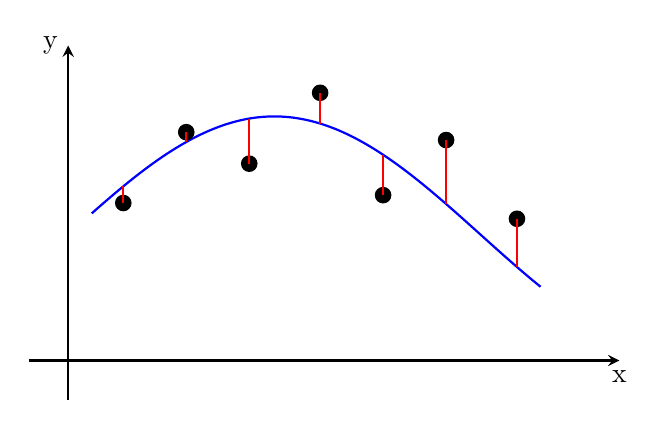
\begin{tikzpicture}[>=stealth, thick]

% ----- Axes -----
\draw[->] (-0.5,0) -- (7,0) node[below] {x};
\draw[->] (0,-0.5) -- (0,4) node[left] {y};

% ----- Regression curve -----
\draw[blue, thick, domain=0.3:6, smooth, samples=200]
  plot(\x,{1.6 + 1.5*sin(0.6*\x r)});

% ----- Data points -----
\foreach \x/\y in {0.7/2, 1.5/2.9, 2.3/2.5, 3.2/3.4, 4.0/2.1, 4.8/2.8, 5.7/1.8}{
  \fill[black] (\x,\y) circle (3pt);
}

% ----- Error lines (real error from curve to point) -----
\foreach \x/\y in {0.7/2, 1.5/2.9, 2.3/2.5, 3.2/3.4, 4.0/2.1, 4.8/2.8, 5.7/1.8}{
  \pgfmathsetmacro{\ycurve}{1.6 + 1.5*sin(0.6*\x r)}
  \draw[red] (\x,\y) -- (\x,\ycurve);
}

% ----- Optional: Label for "Error" -----
% \node[red, font=\bfseries] at (2.2,3.2) {Error};
\end{tikzpicture}
\pause
  \begin{figure}
    \centering
    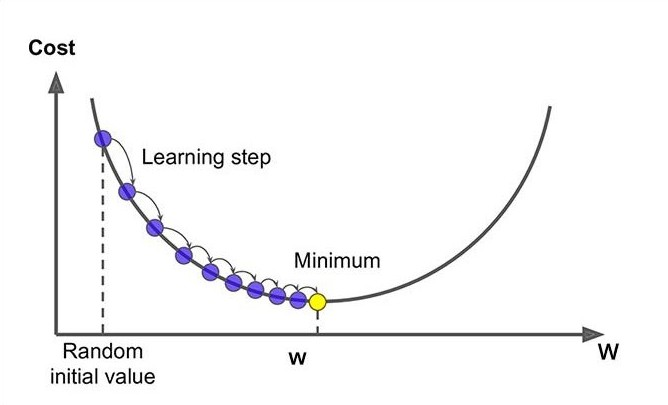
\includegraphics[width=0.49\textwidth]{images/descent.jpg}
  \end{figure}

  \end{center}
  
\end{multicols}



\end{frame}

\section{بازتعریف مسئله و مبانی نظری}

\begin{frame}{مسئله‌ی روزنامه‌فروش}
  \begin{itemize}
    \item ۲۰۰ نفر رزرو کرده‌اند. اگر ۲۰۰ پرس بپزی و ۱۵ نفر نیایند، ۱۵ پرس دور ریخته
      می‌شود، حدود $5.6$ میلیون تومان
    \item اگر ۱۸۵ پرس بپزی و ۱۹۰ نفر بیایند، ۵ دانشجو غذا ندارند — کدام بدتر است؟
    \item جواب کلاسیک (Newsvendor): $\displaystyle \tau^{*} = \frac{C_u}{C_u+C_o}$
      — مقدار بهینه میانگین تقاضا نیست، چندک بحرانی توزیع تقاضاست
  \end{itemize}
  \begin{figure}
    \centering
    
\includegraphics[width=0.72\textwidth]{slides_03_asymmetric_cost}
  \end{figure}
  \note{این همان مسئله‌ای است که در پژوهش در عملیات با نام Newsvendor شناخته می‌شود.
  جمله‌ی کلیدی: اگر کمبود چهار برابر مازاد گران است، آن‌قدر بپز که فقط در $20\%$ مواقع کم
  بیاوری.}
\end{frame}

\begin{frame}{شکست فرمول‌های کلاسیک: نوسان واقعی تا $15.6$ برابر فرضیات نظری است}
  \begin{itemize}
    \item \textbf{رد فرض استقلال افراد:} فرمول‌های تحلیلی غیبت را مستقل می‌دانند (توزیع دوجمله‌ای)، اما رفتار جمعی نوسان را تا $15.6$ برابر فراتر از تئوری می‌برد
    \item \textbf{ماندگاری نوسان پس از کنترل ساختاری:} حتی با کنترل سلف، وعده، تقویم و روز هفته، همچنان $7.6$ برابر نوسان اضافه باقی می‌ماند
    \item \textbf{پیامد راهبردی:} در میان ۷٬۵۷۹ سلول ناهمگن، چندک بهینه فرمول بسته ندارد و باید \textbf{مستقیماً از داده آموخته شود}
  \end{itemize}
  \begin{figure}
    \centering
    
\includegraphics[width=0.55\textwidth]{4.8_variance_vs_res}
  \end{figure}
  \note{در رویکرد کلاسیک پژوهش عملیات، ابتدا یک توزیع پارامتری (مثل دوجمله‌ای با فرض استقلال
  افراد) برازش می‌شود و سپس چندک بهینه تحلیلی حساب می‌شود. اما داده‌ها نشان دادند فرض استقلال
  کاملاً باطل است و نوسان واقعی بین $3.7$ تا $15.6$ برابر فرمول نظری است (بیش‌پراکندگی صعودی).
  حتی کنترل کامل زمان و مکان هم این شکاف را پر نمی‌کند ($7.6$ برابر نوسان اضافه باقی می‌ماند).
  ضمناً ۷٬۵۷۹ سلول مستقل با شرایط متفاوت داریم. نتیجه: چندک نباید از فرمول بسته بیرون بیاید،
  باید مستقیماً از داده یاد گرفته شود. شاهد: \lr{F07}، \lr{F08}، \lr{F09}.}
\end{frame}

\begin{frame}{نیوزوندور داده‌محور و رگرسیون کوانتایل}
  \begin{itemize}
    \item به‌جای «اول توزیع را تخمین بزن، بعد بهینه کن»، مستقیماً تصمیم از داده یاد گرفته
      می‌شود (Ban \& Rudin 2019؛ Huber و همکاران 2019)
    \item ابزار: رگرسیون کوانتایل (Koenker \& Bassett 1978) — تابع زیانی با وزن $\tau$ برای
      کم‌زدن و $1-\tau$ برای زیادزدن
    \item کمینه‌کردن این زیان و حل مسئله‌ی Newsvendor یک کار واحدند، نه دو کار پشت سر هم
  \end{itemize}
  \begin{figure}
    \centering
    
\includegraphics[width=0.68\textwidth]{slides_05_pinball}
  \end{figure}
  \note{مدل مستقیماً «عدد پخت» را می‌آموزد، نه «تقاضا» را. به همین دلیل مدل نهایی یک درخت
  گرادیان‌بوستینگ با هدف کوانتایلی است، همان انتخابی که در رقابت \lr{M5 Uncertainty} هم برنده
  شد. فرمول Pinball را بلند نگو، اسلاید پشتیبان دارد.}
\end{frame}

\begin{frame}{یک تصحیح که مال خود پروژه است}
  \begin{itemize}
    \item فرمول کلاسیک در فضای \textbf{تقاضا} تعریف شده؛ خروجی این پروژه چندکی از
      \textbf{نرخ عدم‌دریافت} است که متمم تقاضاست: $D = Res(1-\rho)$
    \item پس فرمول برمی‌گردد: $\displaystyle \tau^{*}_{\rho} = \frac{C_o}{C_u+C_o}$
    \item تأیید عددی با شبیه‌سازی مستقیم نیوزوندور روی ۴۰۰ هزار نمونه
  \end{itemize}
  \begin{figure}
    \centering
    
\includegraphics[width=0.68\textwidth]{slides_06_tau_mapping}
  \end{figure}
  \note{این اسلاید را حذف نکن، تنها دستاورد نظری قابل‌دفاع پروژه است. سند اولیه‌ی مسئله این
  تبدیل را نداشت؛ با آن نسخه $\tau=0.10$ یعنی کمبود ارزان‌تر از مازاد، دقیقاً برعکس کل
  انگیزه‌ی پروژه. جمله‌ی پایانی: عدد $\tau$ خروجی مدل نیست، ورودی سیاستی است — مدیریت سلف
  نسبت $C_u/C_o$ را تعیین می‌کند و بقیه‌اش خودکار است. شاهد: ردیف ۳۶ decision\_log،
  \lr{reports/tau\_sensitivity.md}.}
\end{frame}

\begin{frame}{داده و قاعده‌ی برش}
  \begin{itemize}
    \item ۲ میلیون رزرو فردی، ۱۴۲ روز سرو، ۳۰ سلف، ۶ شهر
    \item تصمیم پخت ساعت ۱۵ روز قبل برای ناهار و ۲۳ برای شام گرفته می‌شود — مدل فقط چیزی
      را می‌بیند که آن لحظه واقعاً در دسترس بوده
  \end{itemize}
  \begin{figure}
    \centering
    
\includegraphics[width=0.95\textwidth]{slides_07_timeline}
  \end{figure}
  \note{بگو: شام روز قبل، در لحظه‌ی تصمیمِ ناهار فردا هنوز سرو نشده، پس استفاده از آن نشتی
  است با اینکه تاریخش گذشته است. جدول کامل برش به پشتیبان می‌رود — این اسلاید را در ۲۰ ثانیه
  رد شو.}
\end{frame}

\section{آنچه داده گفت}

\begin{frame}{عدم‌دریافت یک تصمیم غذایی نیست، غیبت از دانشگاه است}
  \begin{itemize}
    \item اگر کسی ناهارش را نگیرد، احتمال نگرفتن شامش $3.2$ برابر می‌شود
    \item فرضیه‌ی «ترجیح غذایی شخصی» رد شد: پایداری جفت (فرد، غذا) $0.24$ در برابر پایداری
      خود فرد $0.43$
    \item \textbf{پیامد:} تغییر منو ابزار کاهش هدررفت نیست
  \end{itemize}
  \begin{figure}
    \centering
    
\includegraphics[width=0.55\textwidth]{slides_08_dinner_given_lunch}
  \end{figure}
  \note{شاهد: \lr{F57}، \lr{F55}، \lr{F66}.}
\end{frame}

\begin{frame}{$83\%$ نوسان از یک شوک مشترک روزانه می‌آید}
  \begin{columns}
    \begin{column}{0.5\textwidth}
      \begin{itemize}
        \item تجزیه‌ی واریانس نرخ سلول: $7\%$ نویز نمونه‌گیری، $10\%$ ترکیب رزروکنندگان،
          $83\%$ شوک مشترک روز
        \item در $99.5\%$ جفت‌سلف‌ها این شوک هم‌جهت است — سراسری دانشگاه است نه محلی
        \item خبر خوب: با اطلاعات مجاز در لحظه‌ی برش تا $R^2=0.60$ پیش‌بینی‌پذیر است
      \end{itemize}
    \end{column}
    \begin{column}{0.5\textwidth}
      \begin{figure}
        \centering
        
\includegraphics[width=\textwidth]{slides_09_variance_donut}
      \end{figure}
    \end{column}
  \end{columns}
  \begin{figure}
    \centering
    
\includegraphics[width=0.62\textwidth]{report_14_day_shock_fa}
  \end{figure}
  \note{پیامد: مسئله در سطح «روز دانشگاه» مدیریت می‌شود، نه سطح فرد. شاهد: \lr{F59}، \lr{F60}، \lr{F61}.}
\end{frame}

\begin{frame}{روزهایی که بد به‌نظر می‌رسند، روزهایی نیستند که پول می‌سوزانند}
  \begin{itemize}
    \item همبستگی حجم رزرو با نرخ منفی است ($-0.35$) ولی با هدررفت مطلق شدیداً مثبت
      ($+0.75$)
    \item فهرست «بدترین روزها» با معیار نرخ و با معیار پرس فقط ۴ عضو از ۱۵ عضو مشترک دارند
  \end{itemize}
  \begin{figure}
    \centering
    
\includegraphics[width=0.62\textwidth]{R5_q43_volume_vs_rate}
  \end{figure}
  \note{مهم‌ترین حرف مدیریتی ارائه. شاخص پایش سلف باید «پرس» باشد نه «درصد»، وگرنه مدیریت
  دقیقاً روزهای اشتباه را رصد می‌کند. شاهد: \lr{F80}، \lr{F81}، \lr{F54}.}
\end{frame}

\begin{frame}{هدف‌گیری دانشجویان پرغیبت جواب نمی‌دهد}
  \begin{itemize}
    \item سقف نظری هر سیاستی که $10\%$ افراد را هدف بگیرد، $38\%$ هدررفت است
    \item هدف‌گیری بر پایه‌ی مشخصات جمعیتی به $8.7\%$ می‌رسد — بدتر از انتخاب تصادفی
      ($10\%$)، چون افراد پرنرخ عمدتاً کم‌رزرواند
  \end{itemize}
  \begin{figure}
    \centering
    
\includegraphics[width=0.62\textwidth]{report_12b_lorenz_targeting_fa}
  \end{figure}
  \note{پیامد: هر سیاست جریمه یا محدودیت بر پایه‌ی مقطع، جنسیت یا دوره مبنای داده‌ای ندارد.
  این اسلاید یک ایده‌ی بد را پیش از تولدش می‌کشد. شاهد: \lr{F86}، \lr{F74}، \lr{F73}.}
\end{frame}

\begin{frame}{تقویم سیگنال رایگان می‌دهد}
  \begin{itemize}
    \item روز قبل از تعطیلی: $3.1$ واحد درصد بالاتر، حدود $39\%$ نسبی
    \item چهار روز اول بازگشت پس از وقفه‌ی چهارروزه یا بیشتر: $22\%$ نسبی بالاتر — بدترین
      روز، روز \textbf{دوم} است نه اول
    \item شام رمضان تقریباً دو برابر
  \end{itemize}
  \begin{columns}
    \begin{column}{0.5\textwidth}
      
\includegraphics[width=\textwidth]{report_07_pre_holiday_fa}
    \end{column}
    \begin{column}{0.5\textwidth}
      
\includegraphics[width=\textwidth]{r4_2_return_curve_fa}
    \end{column}
  \end{columns}
  \note{همه‌ی این‌ها ماه‌ها قبل معلوم‌اند و اعمالشان هزینه‌ی صفر دارد، حتی بدون هیچ مدلی.
  شاهد: \lr{F19}، \lr{F70}، \lr{F22}.}
\end{frame}

\begin{frame}{جغرافیا}
  \begin{itemize}
    \item تهران $8.7\%$ در برابر رضوانشهر $3.1\%$، با تفکیک تقریباً کامل بین پردیس‌ها
    \item سازوکارش رفتار افراد است نه ترکیب سلف‌ها — در پردیس دورافتاده سلف تنها گزینه‌ی
      غذایی است
    \item \textbf{پیامد:} تمرکز منابع روی تهران
  \end{itemize}
  \begin{figure}
    \centering
    
\includegraphics[width=0.62\textwidth]{report_02_city_effect_fa}
  \end{figure}
  \note{اگر وقت اضافه داشتی یا استاد پرسید، ماجرای آلودگی هوا را بیاور (\lr{F25}، اسلاید پشتیبان
  پ۱۱): اثر خام قوی بود ($r=+0.28$) و پس از کنترل سلف و وعده کاملاً صفر شد، چون تهران هم‌زمان
  بالاترین آلودگی و بالاترین نرخ را دارد. شاهد: \lr{F12}، \lr{F14}.}
\end{frame}

\section{مدل}

\begin{frame}{چه ساخته شد و مدل به چه چیزی نگاه می‌کند}
  \begin{itemize}
    \item ۱۰۰ ویژگی، ۱۳ خانواده‌ی مدل، غربال چهارمرحله‌ای، انتخاب نهایی یک مدل درختی
      کوانتایلی
    \item پروتکل: تقسیم زمانی با مبدأ غلتان؛ پنجره‌ی آزمون فقط یک‌بار باز شد
    \item مهم‌ترین ورودی‌ها: هویت سلف، برهم‌کنش روزهفته با شهر، حجم رزرو، نرخ دیروزِ همان
      سلول، شوک دیروز
  \end{itemize}
  \begin{figure}
    \centering
    
\includegraphics[width=0.62\textwidth]{9.1_perm_importance_fa}
  \end{figure}
  \note{کلمه‌ی SHAP را نگو، بگو «سهم هر ویژگی در تصمیم مدل». نکته‌ی مهم اینکه این فهرست
  دقیقاً با یافته‌های بخش ۳ می‌خواند، یعنی مدل چیز عجیبی یاد نگرفته. شاهد:
  \lr{reports/phase9/9.2\_shap\_mean\_abs.csv}، \lr{reports/phase7/model\_comparison.md}.}
\end{frame}

\begin{frame}{نتایج منفی}
  \begin{itemize}
    \item از ۲۵ مدل فقط ۵ تا برد آماری معنادار داشتند
    \item شبکه‌های عصبی و مدل سطح فرد کمکی نکردند
    \item قهرمان اعتبارسنجی و قهرمان پنجره‌ی آزمون یکی نبودند، و طبق پروتکل قهرمان عوض نشد
  \end{itemize}
  \begin{figure}
    \centering
    
\includegraphics[width=0.62\textwidth]{slides_15_funnel}
  \end{figure}
  \note{این اسلاید را حذف نکن. استادها روی همین قضاوت می‌کنند. شاهد: یافته‌های ۲۸، ۳۱، ۳۶؛
  ردیف ۴۹ decision\_log.}
\end{frame}

\section{Conclusion}

\begin{frame}{Challenges}
\begin{itemize}
    \item  \textbf{Electric field provided to the model in forward problem}  
    \quad In the paper, the electric field $E(x,t)$ was directly supplied to the PINN during forward training. this may limit the model's ability to infer $E$ self-consistently from the physics.

    \vspace{0.3cm}
    \item  \textbf{Integration in the Poisson equation}  
    \quad The Poisson term $\displaystyle \frac{\partial E}{\partial x} = \int f\,dv - 1$ requires numerical integration.  
    The choice of integration method (e.g., trapezoidal rule) affects stability and accuracy.

    \vspace{0.3cm}
    \item  \textbf{Unknown weighting of loss components}  
    \quad The relative importance of each loss term ($L_{\text{eq}}, L_{\text{IC}}, L_{\text{BC}}$)  
    is not clearly defined-improper weighting can hinder convergence or bias the network.

    \vspace{0.3cm}
    \item  \textbf{Sampling and resampling strategy}  
    \quad The performance strongly depends on how training points are chosen in $(t,x,v)$.  
    Optimal sampling frequency and resampling intervals remain open research questions.
\end{itemize}
\pause
\begin{block}{Observation}
Balancing physical accuracy, numerical stability, and training efficiency  
is still the main challenge for PINN-Vlasov frameworks.
\end{block}
\end{frame}

\begin{frame}{Conclusion}
\begin{itemize}
    \item \textbf{Physics-Informed Neural Networks (PINNs)} bridge the gap between deep learning and physical modeling.
    \item By embedding \textbf{governing PDEs} into the loss function, they ensure physical consistency.
    \item Demonstrated capability for solving both \textbf{forward and inverse problems} with high interpretability.
\end{itemize}
\end{frame}

\begin{frame}{Future Work}
    \begin{itemize}
    \item  \textbf{Improving computational efficiency} — faster training for complex PDEs.
    \item  \textbf{Adaptive sampling} — dynamic selection of collocation points.
    \item  \textbf{Multi-physics extension} — include magnetic fields, collisions, higher dimensions (2D/3D).

\end{itemize}
\vspace{0.5cm}
\pause
\centering
\textit{Future PINNs = Physics + Data + Efficiency → Scientific AI.}
\end{frame}

\backmatter

\section{محدودیت و گام بعد}

\begin{frame}{محدودیت‌ها، با همان دقت نتایج}
  \begin{itemize}
    \item پنج ماه داده، بدون تابستان و بدون سیگنال چندترمی
    \item قیمت ۳۷۵ هزار تومان نرخ امروز است، نه نرخ بازه‌ی داده — و هیچ آزمون میدانی انجام
      نشده
    \item هزینه‌ی کمبود تثبیت نشده، یعنی $\tau$ نهایی یک تصمیم مدیریتی است نه خروجی مدل؛
      نردبان بخش پیش روی فرض تکرار الگوی هفتگی در ۳۲ هفته بسته شده
  \end{itemize}
  \begin{figure}
    \centering
    
\includegraphics[width=0.85\textwidth]{slides_21_calendar_coverage}
  \end{figure}
  \note{شاهد: فصل ۵ گزارش، بند ۵-۲-۲؛ فرضیات صریح \lr{10.4\_annual\_savings.md}.}
\end{frame}

\begin{frame}{پایلوت پیشنهادی}
  \begin{itemize}
    \item دو جفت همتاشده از دو خوشه‌ی پایدار: مدیریت/علوم و کشاورزی/کوی
    \item چهار هفته، ۷۲ مشاهده در هر بازو
    \item این آزمونِ «شدنی‌بودن عملیاتی» است، نه آزمونی با توان آماری کافی
  \end{itemize}
  \begin{figure}
    \centering
    
\includegraphics[width=0.78\textwidth]{slides_22_pilot_pairs}
  \end{figure}
  \note{همین صراحت بیشتر از هر ادعایی امتیاز می‌گیرد. شاهد:
  \lr{reports/phase10/10.5\_pilot\_protocol.md}.}
\end{frame}

\begin{frame}{جمع‌بندی در سه جمله}
  \begin{columns}
    \begin{column}{0.68\textwidth}
      \begin{enumerate}
        \item هر روز سرو، حدود هزار پرس دور ریخته می‌شود؛ سالانه ۲۳۲ هزار پرس و ۸۷ میلیارد
          تومان
        \item با یک تغییر تصمیم — پخت روی چندک به‌جای پخت روی رزرو — $71\%$ آن برمی‌گردد
          ($61.9$ میلیارد تومان در سال) به قیمت $0.28\%$ تقاضای برآورده‌نشده، یعنی ۲۴ پرس
          نجات‌یافته به ازای هر ۱ پرس کمبود
        \item $\tau$ تنها دکمه‌ای است که باید دست مدیریت باشد
      \end{enumerate}
    \end{column}
    \begin{column}{0.30\textwidth}
      
\includegraphics[width=\textwidth]{slides_17_ladder}
    \end{column}
  \end{columns}
\end{frame}

\begin{frame}[c]{\,}
  \centering
  \begin{minipage}{\textwidth}
    \centering
    \Huge سؤال و پاسخ \\[1cm]
    \Large \textsl{با تشکر از توجه شما}
  \end{minipage}
\end{frame}

\section*{اسلایدهای پشتیبان}

\aboutpage{اسلایدهای پشتیبان}{شماره‌گذاری‌شده تا سریع بپری رویشان}

\begin{frame}{پ۱ — تابع زیان Pinball}
  \[
    \rho_\tau(u) = u\left(\tau - \mathbb{1}[u<0]\right), \qquad u = y - \hat y
  \]
  \begin{itemize}
    \item برای $u\ge 0$ (کم‌زدن): شیب $\tau$؛ برای $u<0$ (زیادزدن): شیب $1-\tau$
    \item کمینه‌کننده‌ی امید ریاضی این زیان دقیقاً چندک $\tau$اُم توزیع شرطی $y$ است — اثبات
      با مشتق‌گیری از انتگرال تابع توزیع تجمعی
  \end{itemize}
  {\small شاهد: Literature\_Review.md بند ۲-۲.}
\end{frame}

\begin{frame}{پ۲ — چرا زیان با وزن حجم رزرو وزن‌دهی شد}
  \begin{itemize}
    \item واریانس $\rho$ به‌شدت به اندازه‌ی رزرو وابسته است: std چارک کوچک ÷ بزرگ $=3.03\times$
    \item بدون وزن‌دهی، سلف‌های کوچکِ پرنوسان بر تابع زیان اثر نامتناسب می‌گذارند
    \item راه‌حل: $w=Res$ در تابع زیان
  \end{itemize}
  {\small شاهد: \lr{F06}؛ ردیف ۲۵ decision\_log؛ یافته‌ی ۱۶.}
\end{frame}

\begin{frame}{پ۳ — جدول کامل تبدیل نسبت هزینه به چندک}
  \begin{center}
  \begin{tabular}{cccc}
    \toprule
    $C_u/C_o$ & چندک تقاضا & $\tau_\rho$ (چندک نرخ عدم‌دریافت) \\
    \midrule
    $2\times$ & $0.67$ & $0.33$ \\
    $4\times$ & $0.80$ & $0.20$ \\
    $9\times$ & $0.90$ & $0.10$ \\
    \bottomrule
  \end{tabular}
  \end{center}
  \[
    \tau_\rho = \frac{C_o}{C_u+C_o} = 1 - \frac{C_u}{C_u+C_o}
  \]
  {\small شاهد: \lr{reports/tau\_sensitivity.md}، \lr{reports/phase10/10.2\_newsvendor.md}.}
\end{frame}

\begin{frame}{پ۴ — قاعده‌ی برش اطلاعاتی، کامل}
  \small
  \begin{tabular}{p{5.2cm}p{5.2cm}}
    \toprule
    مجاز & ممنوع \\
    \midrule
    \texttt{Reservation} تا $d+2$ &
      \texttt{ReceiveWithCard/Code}, \texttt{DontReceive} برای روز $d$ \\
    \texttt{Recv/NoRecv}, نرخ $\rho$ تا لحظه‌ی برش همان وعده‌ی هدف &
      هر ستون پس از پخت، و هر وعده که هنوز سرو نشده \\
    منو و ویژگی‌های تقویمی هر روز & — \\
    \texttt{ReserveStatus} تاریخچه‌ی فرد $p$ تا لحظه‌ی برش (مدل B) &
      \texttt{ReserveStatus} برای روز هدف $d$ \\
    \bottomrule
  \end{tabular}
  \vspace{0.2cm}

  تله‌ی رایج: شام روز $d-1$ در لحظه‌ی برش ناهار روز $d$ (ساعت ۱۵) هنوز سرو نشده — با اینکه
  تاریخش $d-1$ است، استفاده از آن نشتی است.
  {\small شاهد: AGENTS.md؛ بند ۴-۲ project-definition.md؛ ردیف ۹ decision\_log.}
\end{frame}

\begin{frame}{پ۵ — هشت خط پایه روی $\tau=0.20$}
  \tiny
  \begin{center}
  \begin{tabular}{lccc}
    \toprule
    خط پایه & pinball & نرخ کمبود & \% کاهش هدررفت \\
    \midrule
    \lr{B3\_empirical\_quantile} & $0.01590$ & $9.6\%$ & $60.1\%$ \\
    \lr{B7\_group\_residual\_quantile} & $0.01591$ & $8.9\%$ & $59.8\%$ \\
    \lr{B2\_group\_shrunk} & $0.01695$ & $9.8\%$ & $54.7\%$ \\
    \lr{B6\_day\_factor} & $0.01744$ & $13.6\%$ & $58.1\%$ \\
    \lr{B1\_global\_mean} & $0.01847$ & $9.9\%$ & $43.4\%$ \\
    \lr{B4\_seasonal\_naive} & $0.02158$ & $11.7\%$ & $43.5\%$ \\
    \lr{B5\_rolling\_mean} & $0.02187$ & $18.3\%$ & $57.8\%$ \\
    \lr{B0\_cook\_all} & $0.02288$ & $0.0\%$ & $0.0\%$ \\
    \bottomrule
  \end{tabular}
  \end{center}
  {\small شاهد: \lr{reports/baselines\_tau020.md}.}
\end{frame}

\begin{frame}{پ۶ — قهرمان در برابر خط پایه، در نقطه‌ی سربه‌سر}
  \begin{itemize}
    \item در $\tau=0.20$ روی پنجره‌ی آزمون، قهرمان از قوی‌ترین خط پایه (\lr{B3}) عملاً چیزی جلو
      نزد: $-0.011$ میلیارد تومان
    \item مزیت مدل در $\tau$های کوچک‌تر ظاهر می‌شود: در $\tau=0.02$ برابر $+0.94$ میلیارد
      تومان
    \item بیشتر ارزش از خودِ سوئیچ به تصمیم چندکی می‌آید، نه از پیچیدگی مدل — مزیت واقعی مدل
      در کالیبراسیون است
  \end{itemize}
  {\small شاهد: \lr{reports/phase10/10.2\_newsvendor.md}.}
\end{frame}

\begin{frame}{پ۷ — اندازه‌ی نمونه‌ی مؤثر و بوت‌استرپ بلوکی دوبعدی}
  \begin{itemize}
    \item اندازه‌ی نمونه: خام $7{,}579$ سلول، مؤثر تنها $593$ (ICC روز $=0.225$) — ضریب
      تورم واریانس $12.8\times$
    \item آزمون‌های آماری فاز ۷ باید روی این اندازه‌ی مؤثر، نه خام، تفسیر شوند
    \item بوت‌استرپ روی هر دو بُعد (روز و سلف) بلوک می‌بندد چون ICC روز و سلف تقریباً برابرند
  \end{itemize}
  {\small شاهد: \lr{reports/baselines\_tau020.md}؛ \lr{F10}.}
\end{frame}

\begin{frame}{پ۸ — بیش‌پراکندگی و رد فرض استقلال افراد}
  \begin{itemize}
    \item در سطح فرد: واریانس گروهی $14.4\times$ دوجمله‌ای؛ $\chi^2/df=18.2$
    \item ICC واحد سکونت $=+0.064$، دانشکده $=+0.033$
    \item \textbf{پیامد حیاتی:} جمع ساده‌ی احتمالات فردی در مدل B عدم‌قطعیت را حدود
      $3.8\times$ کم‌برآورد می‌کند — کوانتایل خوش‌بینانه، ریسک کمبود بیشتر از ادعای مدل
  \end{itemize}
  {\small شاهد: \lr{F08}.}
\end{frame}

\begin{frame}{پ۹ — پنج سطح داده}
  \small
  \begin{center}
  \begin{tabular}{lll}
    \toprule
    سطح & واحد رکورد & حجم \\
    \midrule
    \lr{L1} سلول & $(d,m,r,f)$ & $7{,}579$ \\
    \lr{L2} سلف×وعده & $(d,m,r)$ & حدود $4{,}100$ \\
    \lr{L3} عامل روز & $(d,m)$ & $256$ \\
    \lr{L4} سری زمانی & سری $(m,r)$ & ۴۱ سری، میانه ۱۹۷ نقطه \\
    \lr{L5} رزرو فردی & $(p,d,m,r,f)$ & $2{,}049{,}322$ رزرو \\
    \bottomrule
  \end{tabular}
  \end{center}
  «مدل \lr{A/B}» فازهای ۱ تا ۶: \lr{A} $\equiv$ \lr{L1/L2}، \lr{B} $\equiv$ \lr{L5}.
  {\small شاهد: AGENTS.md.}
\end{frame}

\begin{frame}{پ۱۰ — کالیبراسیون و ACI}
  \begin{itemize}
    \item بدون کالیبراسیون: پوشش تجربی سیستماتیک بیشتر از اسمی است — بیشترین شکاف در
      $\tau=0.30$ ($+18.0\%$)، یعنی مدل محافظه‌کارتر از حد اسمی
    \item در نقطه‌ی عملیاتی $\tau=0.20$: پوشش از $33.6\%$ (شکاف $+13.6\%$) با ACI به
      $20.1\%$ (شکاف $+0.1\%$) می‌رسد
    \item pinball هم کمی بهتر می‌شود: از $0.01008$ به $0.00975$
  \end{itemize}
  {\small شاهد: \lr{reports/phase8/8.8\_calibration.md}.}
\end{frame}

\begin{frame}{پ۱۱ — ماجرای آلودگی هوا}
  \begin{itemize}
    \item اثر خام قوی: $r=+0.28$ ($p\approx 6\times10^{-134}$)
    \item پس از کنترل سلف×وعده×روزهفته: $-0.013$ ($p=0.25$) — کاملاً صفر
    \item سازوکار: تهران هم‌زمان بالاترین AQI و بالاترین نرخ را دارد
  \end{itemize}
  \begin{figure}
    \centering
    
\includegraphics[width=0.6\textwidth]{report_03_aqi_spurious_fa}
  \end{figure}
  {\small شاهد: \lr{F25}.}
\end{frame}

\begin{frame}{پ۱۲ — نمودار کالیبراسیون}
  \begin{figure}
    \centering
    
\includegraphics[width=0.62\textwidth]{8.8_reliability_fa}
  \end{figure}
\end{frame}

\begin{frame}{پ۱۳ — تحلیل باقیمانده}
  \begin{columns}
    \begin{column}{0.5\textwidth}
      
\includegraphics[width=\textwidth]{8.2_residual_hist_fa}
    \end{column}
    \begin{column}{0.5\textwidth}
      
\includegraphics[width=\textwidth]{8.2_resid_acf_fa}
    \end{column}
  \end{columns}
\end{frame}

\begin{frame}{پ۱۴ — درخت جانشین قابل‌فهم}
  \begin{figure}
    \centering
    
\includegraphics[width=0.68\textwidth]{9.5_surrogate_tree_fa}
  \end{figure}
\end{frame}

\begin{frame}{پ۱۵ — منحنی یادگیری}
  \begin{figure}
    \centering
    
\includegraphics[width=0.62\textwidth]{8.9_learning_curve}
  \end{figure}
\end{frame}

\begin{frame}{پ۱۶ — مقایسه‌ی شش مجموعه‌ی ویژگی}
  \begin{figure}
    \centering
    
\includegraphics[width=0.68\textwidth]{5.12_feature_sets_fa}
  \end{figure}
\end{frame}

\begin{frame}{پ۱۷ — خودهمبستگی به تفکیک وعده}
  \begin{figure}
    \centering
    
\includegraphics[width=0.62\textwidth]{report_08_acf_by_meal_fa}
  \end{figure}
\end{frame}

\begin{frame}{پ۱۸ — توزیع متغیر هدف}
  \begin{figure}
    \centering
    
\includegraphics[width=0.6\textwidth]{report_01_target_distribution_fa}
  \end{figure}
\end{frame}

\aboutpage{پرسش‌های محتمل}{جواب کوتاه}

\begin{frame}{«مدل پیچیده چه چیزی بیشتر از یک قاعده‌ی ساده داد؟»}
  خطرناک‌ترین سؤال — خودت اول مطرحش کن (اسلاید ۱۵).
  \begin{itemize}
    \item در $\tau=0.20$ روی پنجره‌ی آزمون، قهرمان از خط پایه‌ی \lr{B3} عملاً چیزی جلو نزد
      ($-0.011$ میلیارد)
    \item بیشتر ارزش از خودِ سوئیچ به تصمیم چندکی می‌آید، نه پیچیدگی مدل
    \item مزیت مدل در $\tau$های کوچک‌تر ظاهر می‌شود ($\tau=0.02$: $+0.94$ میلیارد) و در
      کالیبراسیون
  \end{itemize}
\end{frame}

\begin{frame}{«۶۲ میلیارد چقدر قابل اتکاست؟» / «چرا رگرسیون کوانتایل؟»}
  \begin{itemize}
    \item بازه‌ی $44$ تا $81$ میلیارد با بوت‌استرپ بلوکی، روی ۳۲ هفته‌ی آموزشی، بدون
      تابستان، بدون تورم، بدون رشد ثبت‌نام — فرض‌ها در \lr{10.4\_annual\_savings.md}
    \item تصمیم فقط به یک نقطه از توزیع نیاز دارد؛ تخمین کل توزیع خطای جاهای بی‌ربط را هم
      وارد تصمیم می‌کند
  \end{itemize}
\end{frame}

\begin{frame}{«معادل‌سازی Pinball با نیوزوندور از کجاست؟» / «چرا تک‌مرحله‌ای اجرا نشد؟»}
  \begin{itemize}
    \item Ban \& Rudin (2019)، Huber و همکاران (2019)، صورت‌بندی رسمی در Risks (2026) —
      همان مقاله هشدار می‌دهد کالیبراسیون باید جدا از دقت نقطه‌ای بررسی شود
    \item اجرا شد: خانواده‌ی ۱۱ (\lr{\texttt{f11\_decision.py}}) همین آزمون هم‌ارزی را دارد؛
      نتیجه: هدف واقعی نسخه‌ی وزن‌دار است، نه pinball خام
  \end{itemize}
\end{frame}

\begin{frame}{«هزینه‌ی کمبود را چطور تعیین کردی؟» / «نشتی داده چطور کنترل شد؟»}
  \begin{itemize}
    \item تعیین نشد — این یک تصمیم سیاستی است، نه کمیت قابل‌اندازه‌گیری از داده؛ کل بازه‌ی
      نسبت هزینه از ۲ تا ۴۹ آزموده شد. $\tau=0.20$ توصیه است نه ادعا
    \item نشتی: قاعده‌ی برش به تفکیک وعده با ممیزی خودکار، فولدهای منجمد با دروازه‌ی هش —
      شام روز قبل در لحظه‌ی تصمیمِ ناهار فردا هنوز سرو نشده، پس ممنوع است
  \end{itemize}
\end{frame}

\begin{frame}{«چرا داده‌ی سطح فرد کمک نکرد؟» / «آلودگی هوا واقعاً بی‌اثر است؟»}
  \begin{itemize}
    \item ترکیب افراد فقط $10\%$ واریانس را توضیح می‌دهد، شوک روز $83\%$ — سیگنال فردی
      افزونه بود نه تازه
    \item اثر AQI خام قوی بود، پس از کنترل سلف و وعده صفر شد؛ آزمون آستانه‌ای هم چیزی پیدا
      نکرد — سازوکارش این‌که تهران هم‌زمان بالاترین آلودگی و بالاترین نرخ را دارد
  \end{itemize}
\end{frame}

\begin{frame}{«چرا نرخ کمبود $15.4\%$ ولی مشکلی نیست؟» / «چرا فقط ۵ ماه داده؟»}
  \begin{itemize}
    \item $15.4\%$ فقط رخداد را می‌شمارد نه اندازه را؛ عمق میانگین هر سلول کمبوددار $4.2$
      پرس است
    \item ۵ ماه همان چیزی است که از معاونت دانشجویی تحویل گرفته شد — در محدودیت‌ها آمده و
      اولین قلم کار آینده است
  \end{itemize}
\end{frame}

\begin{frame}{«۲۲۴ روز سرو از کجا آمد؟» / «۲۳۲ هزار پرس با ۱۶۲ هزار پرسِ ۵ ماه نمی‌خواند»}
  \begin{itemize}
    \item ۳۲ هفته‌ی آموزشی = دو نیم‌سال ۱۶هفته‌ای؛ تابستان و نوروز عمداً بیرون گذاشته شدند
      چون الگوی سرو متفاوتی دارند که در این داده مشاهده نشده — هر ترم ۱۱۲ روز سرو
    \item داده‌ی خام $53.4$ ردیف در روز سرو دارد، ولی نردبان روی مبنای فولدهای رسمی با
      $48.5$ ردیف در روز بسته شده — یعنی برآورد محافظه‌کارانه است، نه خوش‌بینانه
  \end{itemize}
\end{frame}

\begin{frame}{«عدد $3.9$ میلیارد فنی امیرآباد چقدر دقیق است؟»}
  \begin{itemize}
    \item برآورد مرتبه‌ی بزرگی است، نه عدد گزارش‌شده در مخزن
    \item از میانگین رزرو این سلف و میانگین پیش‌بینی مدل برای آن، ضرب در ۲۲۴ روز سرو ساخته
      شده — هر دو ورودی از مخزن می‌آیند، ولی خود ضرب در گزارش نیامده
  \end{itemize}
\end{frame}


\end{document}
